\section{Experiments}
\subsection{Optimal Omega}

We first want to focus on finding an optimal value for \(\omega\) to minimize the error given a practical termination condition (see user manual). If we take \(d = 1\) and \(n = 10\), then \(\omega_{\text{opt}}\) is between \(1.3\) and \(1.4\). Interestingly, if we fix \(n\), but change the dimension, the optimal value for \(\omega\) is still between \(1.3\) and \(1.4\), therefore, we can conjecture that \(\omega_\text{opt}\) is not dependent on \(d\). However, it is most definitely dependent on \(n\) since if we keep \(d = 1\), but take \(n = 15\), then \(\omega_{\text{opt}}\) is between \(1.9\) and \(2\).
In essence, this hints that \(\omega_\text{opt}\) increases as \(n\) increases and since we want \(n\) to be large as computationally possible, we want to set \(\omega\) close to \(2\). However, for the following experiments, we will use \(\omega = 1.5\). The justification for these results can be found in \texttt{protocol.py}.

\subsection{Convergence of the Error}

Now the question with probably all numerical methods is, does the error, that is the normed difference of the analytic solution and the approximated one, converge? And indeed, it does. See the graph on figure \ref{fig:boat1}.

\begin{figure}[h]
	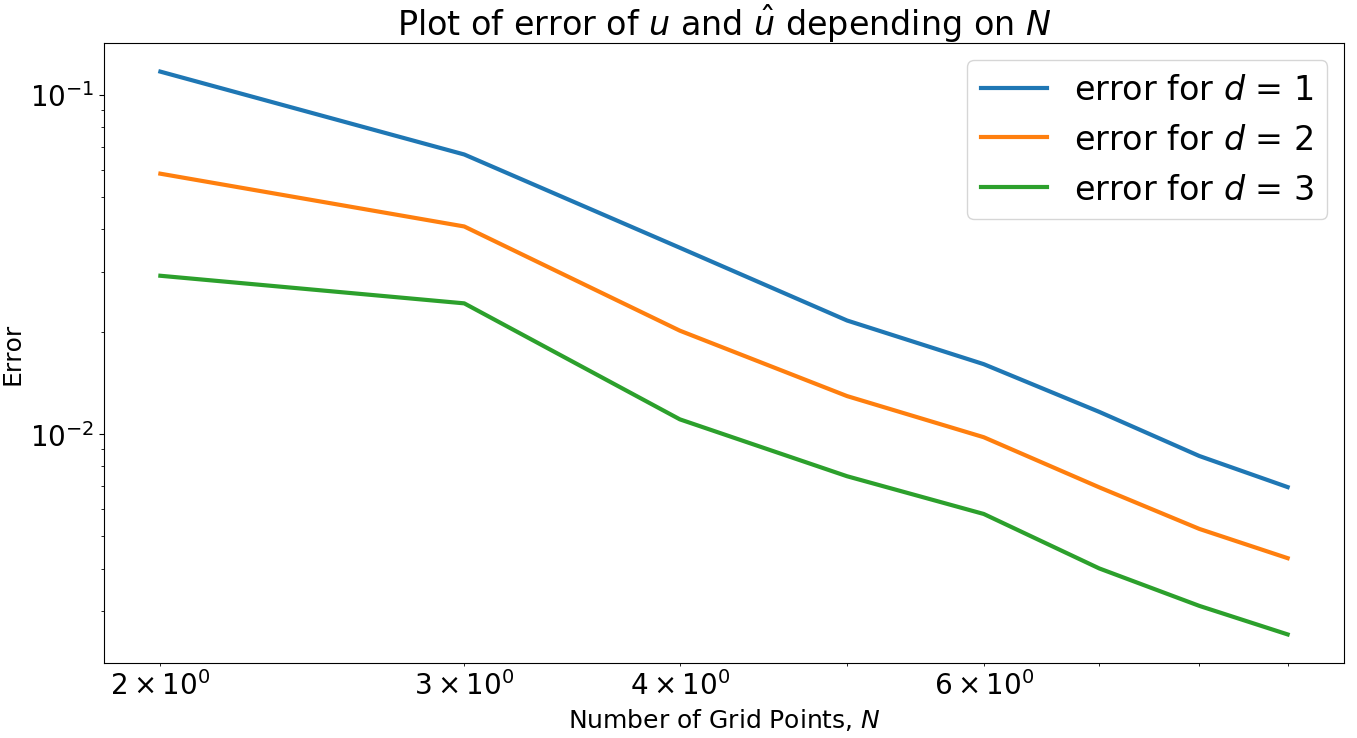
\includegraphics[width=\linewidth]{graphics/error_plot_sor.png}
	\caption{The Error for SOR}
	\label{fig:boat1}
\end{figure}

We can further ask, if the successive over-relaxation method converges faster than solving the system with the LU-decomposition. The visual comparison can be found at figure \ref{fig:boat2} (the plot is only for \(d = 2\) due to the limitation of the working computer of the authors).

\begin{figure}[h]
	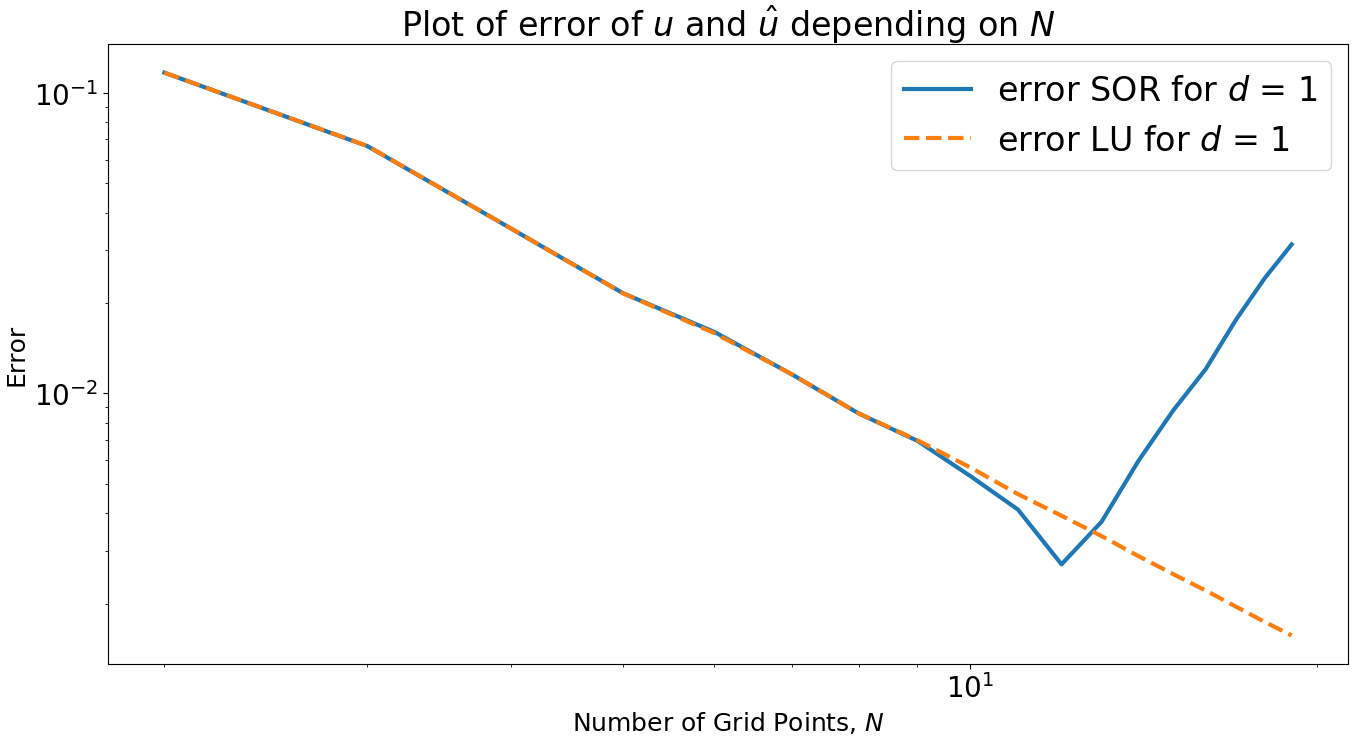
\includegraphics[width=\linewidth]{graphics/plot_error_both.png}
	\caption{The Error for SOR and LU}
	\label{fig:boat2}
\end{figure}

As one can see, the errors are similar on the left side, but at \(n = 12\) the successive over-relaxation becomes better. As the optimal value for \(\omega\) is dependent on \(N\), this means that the SOR algorithm is preferable to the LU-decomposition if a good \(\omega\) can be chosen.